\paragraph{}
Let's begin with the main intuition of the algorithm before expliciting it. For each edge of our polygon, the inside of our simple polygon lies only on one side of this edge. If there exists a point within the polygon from which it is possible to draw a segment to every vertex of the polygon without crossing the boundary of the polygon, then this point must be on the interior-side of each edge. Let's formulate this as a property and then prove it.

\paragraph{}
\textbf{Proposition}

There exists a point within a simple polygon from which it is possible to draw a segment to every vertex of the polygon without crossing the boundary of the polygon \textbf{iff} the intersection of the half-planes defined as the interior-side of each and every edge of the polygon is non-empty.

\paragraph{}
Let's prove it. First, let's assume there exists such a point P. The line between this point and a given vertex is in the inside of the polygon, then this point is on the interior-side of the two edges associated to this vertex. Therefore, this point P has to be on the interior-side of every edge of the polygon.

Reciprocally, let's assume the intersection of the half-planes defined as the interior-side of each and every edge of the polygon is non-empty. Let's consider a point P in this intersection. We need to show that the whole line between this point and any vertex is fully inside the polygon.
Let's consider our line crosses an edge. As our line is going to be inside at its beginning (near P) and at its end (it reaches a vertex by the interior-side of the two edges defining this vertex), it needs to cross at least another edge to re-enter the polygon. This means that our line goes from the outside to the inside of this edge. Therefore P is on the outside-side of this edge which is impossible. Thus, the whole line between P and any vertex is fully inside the polygon.

\begin{figure}[H]
\begin{center}
   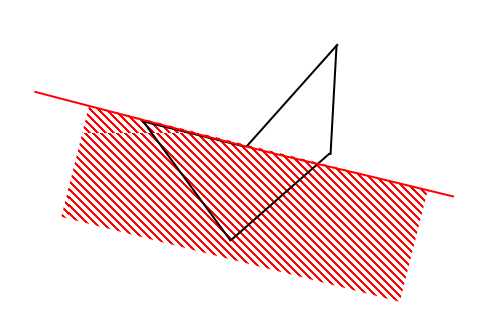
\includegraphics[height=4cm]{fig1.png}
	\caption{illustration of the interior-side half-plane defined by a given edge}
	\label{plot}
	\end{center}
\end{figure}


\paragraph{}
Now that we have found a necessary and sufficient condition for our problem, we can describe an algorithm to solve it using the randomized incremental construction algorithm we saw in class to solve 2D linear optimisation problems. Our algorithm is the following :
\begin{itemize}
	\item We first need to find where is the interior of the polygon given the list of the edges. This is easily done in linear time, for instance by suming the angles knowing that the sum of the interior angles is less than the sum of the exterior ones.
	\item Then we transform our problem into an optimization one, considering that beeing on the interior-side of edge i is giving us an inequality of the form $a_{i,1}x+a_{i,2}y \leqslant b_{i}$. Now we choose a function to optimize, we can take whatever we want so let's pick $f(x,y)=x$. This transformation can be done in time linear to the number of edges.
	\item Finally, we solve this problem with the 2D linear optimisation algorithm seen in class. This algorithm runs in expected linear time. The existence of a solution to the optimisation problem is equivalent to the existence of a point within the polygon from which it is possible to draw a segment to every vertex of the polygon without crossing the boundary of the polygon.
\end{itemize}
 
The three steps of our algorithm run in linear time or expected linear time. Therefore our algorithm runs in expected linear time.
